\documentclass[a4j,12pt]{jsarticle}
\usepackage{semi}
\begin{document}


\日付{2018/07/03}
\氏名{阿部 希駿}
\タイトル{卒業研究}

\semi

\section{緒言}
文部科学省が発表した国際学力調査によると世界の中でも日本の学力は上位にある.しかし日本の学生の学力は二極化していると言われ,問題点は多い.
二極化の下の山の学生は学習内容の一部がわからないのではなく,「何をしているのかがわからない」「どこがわからないのかもわからない」などという根本的な原因があると推測している.

また各塾の調査では中学,高校で学習する科目の中で数学と英語は苦手になりやすいと言われている.この2科目の共通点として既に学習した知識を使うことを前提として授業を行う積み上げ型教科という点がある.積み上げ型教科では単元の内容が複雑になるほど必要な前提知識が多くなり,どの単元の内容が使われているかがわかりにくくなる.そのためその単元の内容を理解をすることが難しくなることが問題点としてあげられる.

そこで「学習する単元を前提知識とする単元の概要をあらかじめ説明することで,内容の理解を促進することができる」という仮説を立てた.
この仮説では特に複数の単元の学習内容を用いて学習を行う単元で,用いる単元の内容などの具体的なイメージがしづらい場合を対象にする.
本研究では,講義にて学生を対象にして実験を行い,この仮説を検証することを目的とする.
講義では「ブロックチェーン」を対象にする.学習の過程である「暗号」や「ハッシュ」の段階では計算などの学習がメインで目的がわかりづらいが,「ブロックチェーン」では

\newpage
\section{教科の特性}
学校で学習する教科には独立型教科と積み上げ型教科に分かれ,それぞれ下図のように積み木のような図で表される.

\begin{figure}[H]
\centering
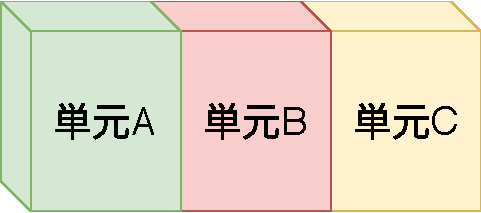
\includegraphics[width=7cm]{02.pdf}
\caption{独立型教科の教育モデル}
\label{fig:02}
\end{figure} 

\begin{figure}[H]
\centering
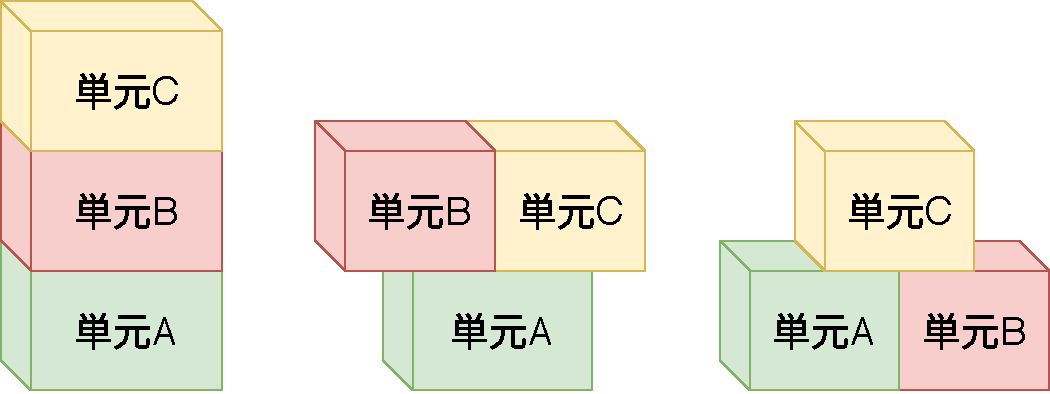
\includegraphics[width=12cm]{03.pdf}
\caption{積み上げ型教科の教育モデル}
\label{fig:03}
\end{figure} 


\subsection{独立型教科}
独立型教科は国語や社会が該当する.
独立型教科では図\ref{fig:01}のように各単元が独立していて関連性があまりないためどの単元から学習しても支障がない.
\begin{figure}[H]
\centering
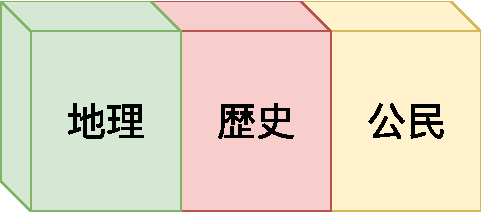
\includegraphics[width=6cm]{01.pdf}
\caption{独立型教科の例}
\label{fig:01}
\end{figure} 

\subsection{積み上げ型教科}
積み上げ型教科では数学や英語が該当する.
積み上げ型教科では図\ref{fig:04}のように学習した内容を次の学習の基礎知識として用いるため,順番に学習していくことになる.

\begin{figure}[H]
\centering
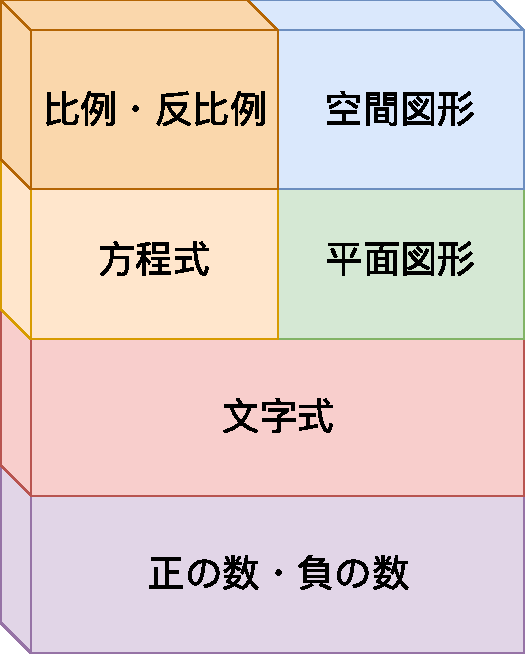
\includegraphics[width=5cm]{04.pdf}
\caption{積み上げ型教科の例}
\label{fig:04}
\end{figure} 

\newpage
\section{暗号について}
暗号とは通信を行う際,第三者にその内容を知られないようにするための手段である.
元の文に一定の規則を用いて特定の変形を加えることを暗号化,暗号化する前の元の文を平文,暗号から平文に戻すことを復合化(復号)と呼ぶ.
暗号化する手段が暗号アルゴリズムであり,また暗号化や復号化に使うデータを鍵と呼ぶ.
暗号は特性によって古典暗号と現代暗号に分かれる.
アルゴリズムがわかれば解読が容易になる暗号を古典暗号,アルゴリズムは公開するが鍵を非公開にすれば安全な暗号を現代暗号という.

\subsection{共通鍵暗号}
暗号化と復号に同じ鍵を用いる暗号の方式である.
通信相手に鍵を送り,その鍵を用いて情報を暗号化する.
暗号化された情報が送られてきたら,同じ鍵を使って復号する.


\begin{figure}[H]
\centering

\includegraphics[width=9cm]{noimage.pdf}
\caption{共通鍵暗号通信の流れ}
\label{fig:no}
\end{figure} 

共通鍵暗号通信では暗号化と同じ鍵を使っているため,鍵を送る際に第三者に傍受される危険がある.
また同じ鍵を複数のユーザーで使用すると,他のユーザーが復号する危険性があるため,ユーザーごとに鍵を生成する必要がある.



\subsubsection{換字式暗号の仕組みと例}
平文の文字を他の記号や文字に置き換えて暗号文を作る古典暗号の方式である.
換字式暗号の代表としてシーザー暗号がある.
シーザー暗号は鍵である決められた文字数分のアルファベットをずらして暗号化を行う.
図\ref{fig:05}は鍵が1であるときの例である.

\begin{figure}[H]
\centering
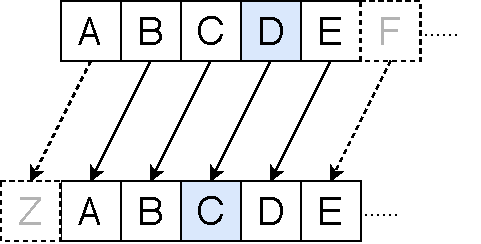
\includegraphics[width=9cm]{05.pdf}
\caption{シーザー暗号の例}
\label{fig:05}
\end{figure} 


\subsubsection{転置式暗号の仕組みと例}
平文の位置を並び替えて暗号文を作る古典暗号の方式である.
転置式暗号の代表としてスキュタレー暗号がある.
スキュタレー暗号はスキュタレーと呼ばれるシリンダーに細長い紙を巻きつけ,平文を横書きに書く.
紙をスキュタレーから外すと順番が入れ替わった暗号ができる.
暗号の受け取る側は同じ半径のスキュタレーを用意し,紙を巻きつけることで復号することができる.
この場合,鍵は同じ直径であることである.

\begin{figure}[H]
\centering
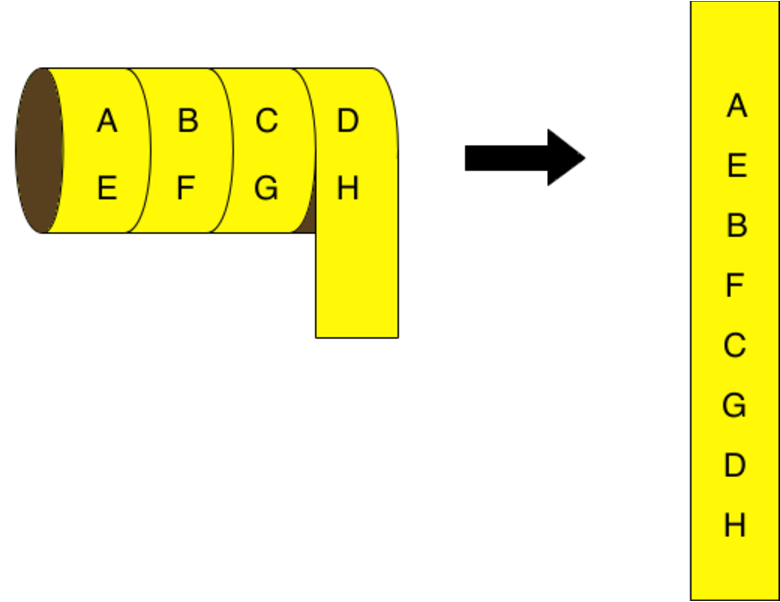
\includegraphics[width=9cm]{062.pdf}
\caption{スキュタレー暗号の例}
\label{fig:06}
\end{figure} 



\subsection{公開鍵暗号}

暗号化と復号に別の手順を用いる暗号方式である.
ユーザは秘密鍵から公開鍵を生成する.
通信相手に送る鍵を公開鍵と呼び,自分の手元に保管しておく鍵を秘密鍵と呼ぶ.
公開鍵を通信相手に送り,通信相手は公開鍵を使って情報を暗号化する.
ユーザは受け取った暗号化された情報を秘密鍵を用いて復号する.

公開鍵暗号では「閉じることはできても開けることができないこと」を安全の根拠としており,一方向関数である素因数分解や楕円曲線が使われる.



\begin{figure}[H]
\centering

\includegraphics[width=9cm]{noimage.pdf}
\caption{公開鍵暗号通信の流れ}
\label{fig:no}
\end{figure} 

公開鍵暗号は共通鍵暗号とは違い各ユーザーごとに鍵を生成する必要がない.
また鍵の受け渡しの際に傍受される可能性がある共通鍵暗号通信とは違い,公開鍵では復号することができない.そのため共通鍵暗号通信よりも安全性が高い.しかし復号に複雑な計算を用いるため負荷が大きくなるため通信に時間がかかるという欠点もある.


公開鍵暗号の代表的な方式であるRSA暗号など電子署名の役割を持つ暗号方式もある.
RSA暗号など公開鍵と秘密鍵が同じ構造をしている暗号では,どちらの鍵を使っても暗号化することができる.
そのため秘密鍵で暗号化し,公開鍵で復号することによって.送信者が本人である根拠とする.

\begin{figure}[H]
\centering

\includegraphics[width=9cm]{noimage.pdf}
\caption{公開鍵暗号における電子署名の流れ}
\label{fig:no}
\end{figure} 




\subsubsection{RSA暗号の仕組みと例}
RSA暗号は桁数の多い素数の掛け算をするのは簡単だが,その合成数の素因数分解をするのは困難であることを安全性の根拠とした公開鍵暗号の一つである.



\subsection{SSL暗号化通信の仕組み}
共通鍵暗号方式は公開鍵暗号方式よりも負荷が小さいが,鍵の受け渡し時に傍受される危険性があった.
そこで鍵の受け渡し時に公開鍵暗号方式を用いることで安全性を確保したものがSSL暗号化通信である.

SSL暗号化通信ではまずユーザが通信相手に接続要求をする.
通信相手から送られてきた公開鍵を使って共通鍵を暗号化し,通信相手に送付する.
通信相手は暗号化された共通鍵を秘密鍵を使って復号する.
これで共通鍵が安全に通信相手に渡ったので,共通鍵暗号通信で情報を送ることができる.



\begin{figure}[H]
\centering

\includegraphics[width=9cm]{noimage.pdf}
\caption{SSL暗号化通信の流れ}
\label{fig:no}
\end{figure} 



\subsection{暗号の歴史}






\newpage
\section{ハッシュ化について}

データを固定長の値であるハッシュ値に不可逆変換して置き換えることである.
ハッシュ値は一定の法則で短縮されているため,違うデータを同じハッシュ値になるように改ざんするのは困難である.
そのためファイルの改ざんや破損の検知,同一性確認などに使用される.

\newpage
\section{ブロックチェーンについて}

\newpage
\section{実験}
本章では,提案した仮説が正しいことを証明するために実験を行う.以下で実験方法の解説を行う.
\subsection{実験目的}
本研究で提案した「学習する単元を前提知識とする単元の概要をあらかじめ理解することで,内容の理解を促進することができる」という仮説が正しいことを証明することを目的とする.

\subsection{実験方法}
\subsubsection{実験対象}

千葉工業大学 情報科学部 情報ネットワーク学科の学生のうち

2018年後期に開講された情報数学応用の受講者

1限76名,2限76名,計152名

ただし複数回の講義を用いての実験であるため,比較や分析に使用するデータは小テスト受験者のみである.


\subsubsection{実験期間}

情報数学応用の講義にて3週かけて行う.

1週目:平成30年11月16日

2週目:平成30年11月30日

3週目:平成30年12月7日



\subsubsection{実験方法}

1限では仮説を用いた講義を行い,2限では仮説を用いない講義を行う.最後に両クラスで同一の小テストを行い,点数の比較と分析を行う.
また小テストと同じ用紙にてアンケートを行う.

(1)講義スケジュール

実験を行う講義は図\ref{fig:timeline}のように行う.
仮説を用いた1限の講義では最初に暗号とハッシュを前提知識とするブロックチェーンの概要について学習した後に,暗号とは負について学習する.
仮説を用いない2限の講義では最初に暗号とハッシュについて学習した後に,ブロックチェーンについて学習し始める.
\begin{figure}[H]
\centering
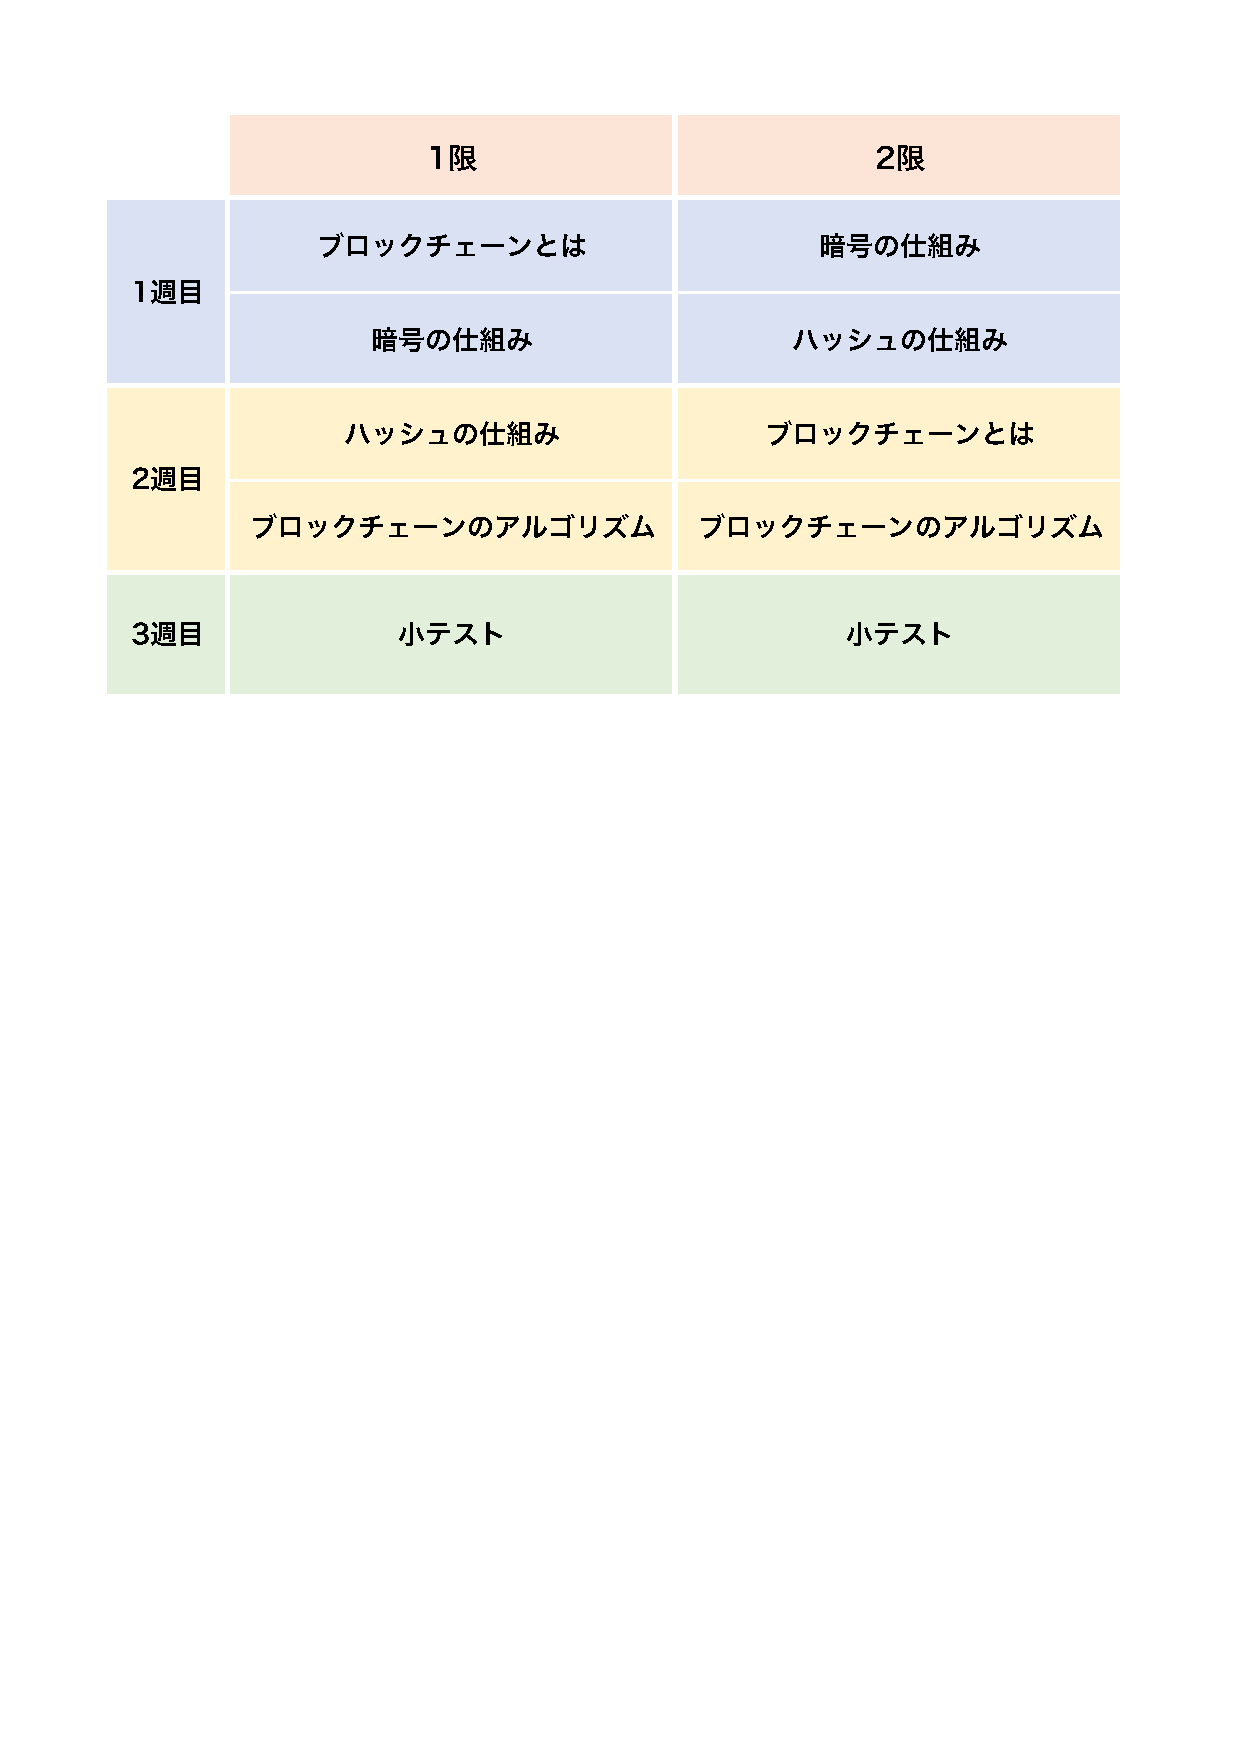
\includegraphics[mediaboxonly=/CropBox,width=12cm]{timeline.pdf}
\caption{講義スケジュール}
\label{fig:timeline}
\end{figure} 


(2)小テスト内容

小テストでは以下の内容を問う.

\UTF{2460}RSA暗号の特徴

\UTF{2461}ハッシュと暗号の違い

\UTF{2462}ブロックチェーンの仕組み

点数配分は\UTF{2460}+\UTF{2461}で5点,\UTF{2462}で5点の合計10点とする.\\


(3)アンケートについて

「ブロックチェーンについて講義を受ける前に学習したことがあるか」について「はい」「いいえ」の二択で聞いた.
「はい」と答えた学生は仮説の「あらかじめ内容を理解する」に該当するが,人数に偏りができることと,元の知識により高得点を取る可能性が高いことから,比較の対象とはせず参考程度に留めることとする.

またアンケート未回答の学生も比較の対象としないこととする.

\newpage
\section{実験結果}
\subsection{アンケート結果と分析対象者}
各クラスのアンケートの結果は表\ref{fig:ank}のようになった.

\begin{table}[H]
\centering
\begin{tabular}{|c|c|c|}
\hline
\multicolumn{1}{|l|}{} & \multicolumn{1}{l|}{1限} & \multicolumn{1}{l|}{2限} \\ \hline
学習したことがない              & 56                      & 60                      \\ \hline
学習したことがある              & 4                       & 4                       \\ \hline
アンケート未回答               & 2                       & 3                       \\ \hline
小テスト未受験                & 14                      & 9                       \\ \hline
\end{tabular}
\caption{アンケート結果}
\label{fig:ank}
\end{table}


\subsection{小テストの点数の比較}

\newpage
\section{考察}

\newpage
\section{結言}

\section{参考文献}

\section{謝辞}

\section{付録}

\end{document}
